\documentclass[british,12pt]{phdthesis}
\bibliographystyle{phdthesis}
\usepackage[british]{babel}

\usepackage{numprint}
\npthousandsep{,}\npthousandthpartsep{}\npdecimalsign{.}

%\usepackage[toc, nonumberlist]{glossaries} % glossaries before hyperref to avoid linking.

\usepackage{multirow}
\usepackage[draft]{varioref}
\usepackage[english,vario]{fancyref}
\usepackage{setspace}

%\usepackage[none]{hyphenat} % debug: hypthenation off

%
\usepackage{tikz}
\usetikzlibrary{shapes,arrows}
\usepackage{minibox}
%\usepackage{epstopdf} % eps to pdf 
\usepackage{graphicx}
\usepackage{algorithm2e}
\usepackage{pgfplots}
%\pgfplotsset{compat=1.13}
\usepackage{array,booktabs,xcolor}
\usepackage{subfigure}
\usepackage{common}
\usepackage{tabu}
\usepackage{verbatim}
\usepackage{array}
%\newcolumntype{L}{>{\centering\arraybackslash}m{2cm}}
\usepackage{colortbl}
\usepackage{url}
\usepackage{wrapfig}
\newcommand{\clust}[2][k]{#2^{\{#1\}}}
\usepackage[labelfont=bf]{caption}
\usepackage{floatrow}
\usepackage{epsfig}

%% A small-ish font size for tables.
\makeatletter
\newcommand\tablefont{\@setfontsize\tablefont{8.5pt}{8.5}}
\makeatother

% Space after captions
\setlength{\belowcaptionskip}{2em}

%

\def\@firstoftwo@second#1#2{%
  \def\temp##1.##2\@nil{##2}%
   \temp#1\@nil}
\newcommand\sref[1]{%
   \expandafter\@setref\csname r@#1\endcsname\@firstoftwo@second{#1}%
}

\def\etal{et~al.\,}
 
%papers:
\newif\ifincpapers
%\incpapersfalse
\incpaperstrue

% chapters
\newif\ifincchapters
%\incchaptersfalse
\incchapterstrue

\usepackage{pdfpages}
\setboolean{@twoside}{false} 
%\pgfpagesuselayout{resize to}[a4paper]

\usepackage{pdflscape} % or rotate figure?
% backref=page % page number of where citation appears.

%\usepackage[backend=bibtex]{biblatex}
%\NewBibliographyString{backrefpages}
%\NewBibliographyString{backrefpages}
%\DefineBibliographyStrings{english}{%
%    backrefpage  = {\lowercase{s}ee p.}, % for single page number
%    backrefpages = {\lowercase{s}ee pp.} % for multiple page numbers
%}

\PassOptionsToPackage{hyphens}{url}\usepackage[hidelinks,pagebackref]{hyperref} % [hidelinks,backref=page]{hyperref}
\def\UrlBreaks{\do\/\do-}
\renewcommand*\backref[1]{\ifx#1\relax \else (Cited on page #1) \fi}

% Invisible section for paper titles:
\newcommand\invisiblesection[1]{\refstepcounter{section}%
\addcontentsline{toc}{section}{\protect\numberline{\thesection}#1}\sectionmark{#1}}

% Invisible subsection for intro
\newcommand{\hiddensubsection}[1]{
\stepcounter{subsection}
\subsection*{\arabic{chapter}.\arabic{section}.\arabic{subsection}\hspace{1em}{#1}}
}
 
%\bibliographystyle{abbrv}

\title{Thesis Title Template: A generic title.}
\author{Author Name}

\authoraddress{
        School of Computer Science \\
        University College Dublin, \\
        Belfield, Dublin 4, Ireland}

\date{\today}

\submission{This thesis is submitted to University College Dublin in fulfilment of the requirements for the degree of Doctor of Philosophy}

\department{School of Computer Science}
\hod{P\'{a}draig Cunningham}

\supervision{Dr. Super Visor 
\secondsupervisor{Professor Second Supervisor}
\doctoralpanel{
External Examiner: Prof. External Examiner\\
Internal Examiner: Dr. Internal Examiner\\
Chair of the Examination Committee:	Prof. Committee Chair 
}
}

\submissionmonth{September}
\submissionyear{2020}

%\makeglossaries
%\renewcommand{\glossarypreamble}{
%This glossary draws together a collection of definitions which will be introduced and discussed later in the text. This list acts as a reference, for the convenience of the reader.
%}
%\newglossaryentry{a glossary entry}
%{
%  name=The Entry,
%  description={A description of the entry}
%}
%#############################END:GLOSSARY

\begin{document}

\maketitle

%% These are optional

%\listoftables

%\listoffigures

%\printglossaries

\begin{dedication}
Statement of Authorship

I hereby certify that the submitted work is my own work, was completed while registered as a candidate for the degree stated on the Title Page, and I have not obtained a degree elsewhere on the basis of the research presented in this submitted work.

\vspace{5 cm}

Signature\hspace{0.5cm} \makebox[2in]{\hrulefill}
\end{dedication}

\begin{dedication}
Dedication goes here.
\end{dedication}

%#############################BEGIN:ACK
\begin{acknowledgements}

Acknowledgements.

\end{acknowledgements}
%#############################END:ACK

\newpage

%This work is supported by \textbf{Science Foundation Ireland} under Grants No. [08/SRC/I1407, SFI/12/RC/2289]. (Clique: Graph and Network Analysis Cluster, and Insight: Centre for Data Analytics).

%%%%%%%%%%%%%%%%%%%%%%%%
% Alternative way of presenting publications:
%\begin{listofpublications}
%\label{listofpublications}
%\begin{itemize}
%\item Surname, Initial. and Surname, Initial. \textbf{Paper Title}. In: Conference Title. %Conference Location, Conference Date. 
%\end{itemize}
%\end{listofpublications}

\onehalfspacing

%%%%%%%%%%%%%%%%%%%%%%%%%%%%%%%%%%%%%%%%%%%%%%%%%%%%%%%%%%%%%%%%%%%%%%%%%%

\begin{abstract}
\label{ch:abstract}
Abstract text, to fill a page.
\end{abstract}

%%%%%%%%%%%%%%%%%%%%%%%%%%%%%%%%%%%%%%%%%%%%%%%%%%%%%%%%%%%%%%%%%%%%%%%%%%%%%
\setcounter{secnumdepth}{2}

\tableofcontents

%%%%%%%%%%%%%%%%%%%%%%%%%%%%%%%%%%%%%%%%%%%%%%%%%%%%%%%%%%%%%%%%%%%%%%%%%%%%%

\pagenumbering{arabic}
\addtocontents{toc}{\protect\setcounter{tocdepth}{2}}

\chapter{Introduction}
\label{ch:introduction}
\ifincchapters
Intro 

\section[Aims and Overview]{Aims}
\label{invisible:aimsoverview}

Aims

\section*{Overview}

Overview

\section{Intro}
\label{sec:intro2}

More Intro 
\fi

\section{Intro Section}
\label{sec:introsub}

%%%%%%%%%%%%%%%%%%%%%%%%%%%%%%%%%%%%%%%%%%%%%%%%%%%%%%%%%%%%%%%%%%%%%%%%%%%%%

\section{Contributions}
\label{ch:contributions}
\ifincchapters
%\addcontentsline{toc}{subsection}{\protect\numberline{}Publications}%

The chapters in this thesis are based on the following articles:

\subsection{Publications}

\begin{itemize}

\item \ref{paper:one} \textbf{First Author}, Second Author, Third Author --- \emph{A paper title} \cite{10.1371/journal.pcbi.1005619} proceedings of the something ABC conference on Foo Bar (Foobar). 

F.A. wrote the manuscript in consultation with S.A. and T.A.

\item \ref{paper:two} \textbf{First Author}, Second Author, Third Author --- \emph{A paper title} \cite{morley2014academic} proceedings of the something ABC conference on Foo Bar (Foobar).

F.A. developed the system. F.A. and S.A. contributed to the design and implementation of the research, T.A. contributed to the evaluation. F.A. wrote the manuscript in consultation with S.A. and T.A.

\end{itemize}

\pagebreak

%\addcontentsline{toc}{subsection}{\protect\numberline{}Supplementary Materials}%
\subsection{Supplementary Materials}

Supplementary materials related to the publications in this thesis include: 

\begin{itemize}

\item Dataset \cite{puschel2008small} used in Section \ref{ch:main1}.

\end{itemize}

These publications have emanated from research conducted with the support of Science Foundation Ireland (SFI) under Grant Numbers 08/SRC/I1407, SFI/12/RC/2289, 07/CE/I1147

%\addtocontents{toc}{\protect\pagebreak}

\fi

%%%%%%%%%%%%%%%%%%%%%%%%%%%%%%%%%%%%%%%%%%%%%%%%%%%%%%%%%%%%%%%%%%%%%%%%

\chapter{Main Thesis Body}
\label{ch:main1}
\ifincchapters
Research. Papers. Etc.

\section{Paper One}
\label{paper:one}

A chapter section based on a paper \cite{morley2014academic}.

\begin{figure}
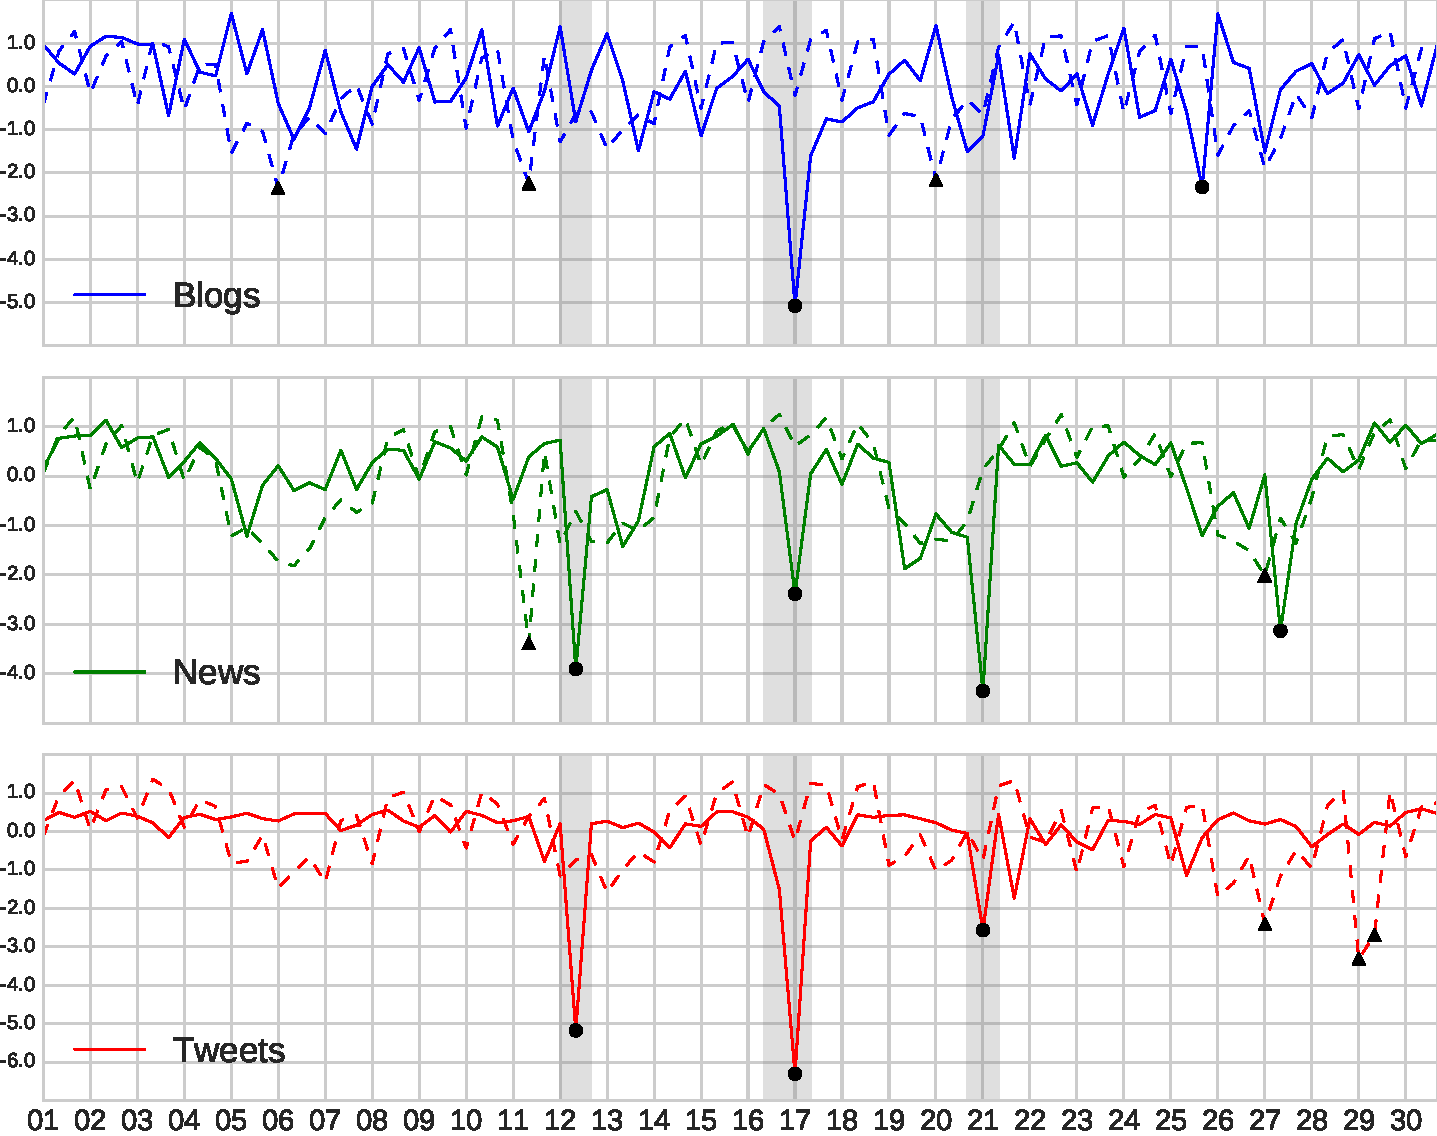
\includegraphics[width=\textwidth]{figures/trump.pdf}
\caption{A Picture}
\label{fig:picture}
\end{figure}

\section{Paper Two}
\label{paper:two}

A chapter section based on another paper

\begin{table}
\caption{Tabular Data}
\label{tbl:table}
\end{table}
\fi
\newpage

%%%%%%%%%%%%%%%%%%%%%%%%%%%%%%%%%%%%%%%%%%%%%%%%%%%%%%%%%%%%%%%%%%%%

\chapter{Conclusions}
\label{ch:conclusions}
\ifincchapters
Chapter \ref{ch:introduction} outlined the importance of bla.

\fi
\newpage

%%%%%%%%%%%%%%%%%%%%%%%%%%%%%%%%%%%%%%%%%%%%%%%%%%%%%%%%%%%%%%%%%%%%

%\part*{Appendices}
%\chapter{Appendix 1}
%\addcontentsline{toc}{chapter}{\protect\numberline{}Appendix}%
%\appendix
%\section{Test}

\singlespacing

\bibliography{main}
\newpage
\phantom{a}

\begin{figure}[b]
  \centering
	
\includegraphics[height=3cm]{graphics/logos/SFI.png} %\hspace{0cm}
	\hfill
	
\includegraphics[height=3cm]{graphics/logos/ucd_brandmark_colour.jpg}%\hspace{0cm}
	\hfill
	
\includegraphics[height=3cm]{graphics/logos/insightlogo.pdf} %\hspace{0cm}
\end{figure}

\end{document}
